% Секция 2.3: Анализ коллективной активности искусственной РНС
% Источник: Kononov2025 (arXiv, на рецензии в Neurocomputing)

\section{Анализ коллективной активности искусственной рекуррентной нейронной сети}\label{sec:rnn}

\link{Связка: коллективные переменные возникают и в искусственных нейронных сетях, особенно в тех, где внутренняя динамика достаточно богата для формирования аттракторов. Мы проверяли, можно ли из коллективной активности рекуррентной нейронной сети сделать вывод о механизмах принятия решения и определить, как алгоритм обучения влияет на вычислительную стратегию сети.}

В данной секции описаны результаты, полученные в работе~\cite{Kononov2025}. Было проведено систематическое сравнение рекуррентных нейронных сетей, обученных методами обучения с подкреплением (ОП) и обучения с учителем (ОУ) на идентичной задаче контекстно-зависимого принятия решений. Показано, что при одинаковой поведенческой эффективности оба алгоритма приводят к качественно различным внутренним вычислительным механизмам.


\subsection{Задача контекстно-зависимого принятия решений}

Использовалась рекуррентная нейронная сеть (РНС) с $N = 250$ скрытыми нейронами (ReLU), 7 входами и 3 выходными действиями (фиксация, выбор~1, выбор~2). Динамика скрытого состояния определялась уравнением
\begin{equation}
\mathbf{h}_{t+1} = \text{ReLU}(\mathbf{W}_{hh} \mathbf{h}_t + \mathbf{W}_{ih} \mathbf{I}_t),
\label{eq:rnn_update}
\end{equation}
где $\mathbf{h}_t \in \mathbb{R}^{250}$~--- вектор скрытого состояния, $\mathbf{I}_t \in \mathbb{R}^{7}$~--- входной вектор, $\mathbf{W}_{hh}$~--- матрица рекуррентных весов, $\mathbf{W}_{ih}$~--- матрица входных весов.

Сеть решала задачу контекстно-зависимого принятия решений (CtxDM)~\cite{Mante2013}: агент должен интегрировать один из двух зашумлённых стимулов, выбирая релевантный на основании контекстного сигнала. Каждая проба состояла из четырёх фаз: фиксация, предъявление стимула, задержка и принятие решения. Входной вектор кодировал сигнал фиксации, два стимульных канала для каждого контекста (когерентности $coh_A = A_1 - A_2$ и $coh_B = B_1 - B_2$, $\in [-1, 1]$) и два контекстных указателя.

Обучение проводилось двумя алгоритмами. ОП использовало алгоритм Proximal Policy Optimization (PPO) с вознаграждением $+1$ за правильное решение и $-1$ за ошибку. ОУ использовало оптимизатор Adam с функцией потерь на основе кросс-энтропии. Оба алгоритма позволяли достичь точности выше 95\% на тестовой выборке, однако анализ внутренней динамики показал качественные различия в вычислительных стратегиях сетей (рис.~\ref{fig:rnn_task}).

\begin{figure}[ht]
\centering
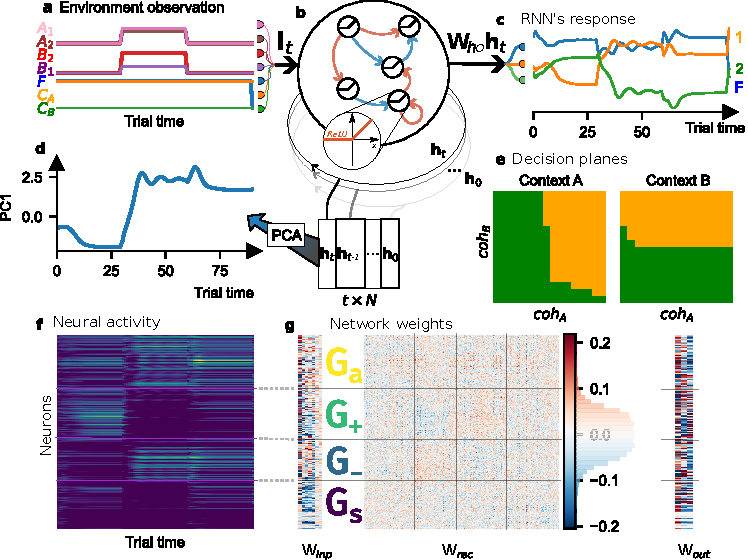
\includegraphics[width=\textwidth]{images/rnn/fig1_task.pdf}
\caption{Структура задачи и архитектура обученной РНС.
(a)~Временн\'{а}я структура пробы: фиксация, стимул, задержка, решение.
(b)~Архитектура РНС ($N=250$ нейронов).
(c)~Выходные вероятности обученной сети в ходе пробы.
(d)~Первая главная компонента активности скрытого слоя.
(e)~Границы решений в двумерном пространстве когерентностей.
(f)~Растровая диаграмма активности скрытого слоя.
(g)~Матрица рекуррентных весов, упорядоченная по функциональным популяциям: сильное внутрипопуляционное возбуждение и межпопуляционное торможение. Эта структура не была задана заранее, а возникла в результате обучения.
По~\cite{Kononov2025}.}
\label{fig:rnn_task}
\end{figure}


\subsection{Многоуровневый анализ популяционной активности}\label{sec:rnn_methods}

Для систематического сравнения внутренних механизмов сетей, обученных ОП и ОУ, был разработан многоуровневый аналитический подход, объединяющий три взаимодополняющих уровня анализа.

\textit{Уровень~1: классификация аттракторов.} Для идентификации типов аттракторов длительность стимульной фазы продлевалась до 1000 шагов, что позволяло динамике системы достичь стационарного состояния. Поскольку активационная функция ReLU задаёт кусочно-линейную динамику, для каждого набора активных нейронов $\mathcal{A}$ тип аттрактора определялся по собственным значениям подматрицы весов $\mathbf{W}^{\mathcal{A}}_{hh}$: при $|\mu_{lead}| < 1$~--- устойчивая неподвижная точка, при $|\mu_{con}| > 1$ для пары комплексно-сопряжённых собственных значений~--- квазипериодический аттрактор.

\textit{Уровень~2: популяционная классификация.} Нейроны классифицировались по функциональным группам с помощью метода сопоставления с шаблонами (template matching). Для каждого нейрона строилась матрица активности по пространству когерентностей, а затем вычислялось расстояние до четырёх канонических шаблонов:
\begin{equation}
c^* = \argmin_{c \in \{\mathrm{G}_s,\mathrm{G}_+,\mathrm{G}_-,\mathrm{G}_a\}} \sum_{i,j} (M^{(n)}_{i,j}-M^{c}_{i,j})^2,
\label{eq:rnn_population}
\end{equation}
где $\mathrm{G}_s$~--- молчащие нейроны, $\mathrm{G}_+$ и $\mathrm{G}_-$~--- нейроны, селективные к положительной и отрицательной когерентности, $\mathrm{G}_a$~--- нейроны, активные при любом стимуле.

\textit{Уровень~3: информационно-теоретический анализ.} Функциональные роли популяций верифицировались с помощью взаимной информации между активностью отдельных нейронов и переменными задачи; подробный анализ и результаты представлены в секции~\ref{sec:intense_rnn}.

Для визуализации высокоразмерных нейронных траекторий использовался автоэнкодер ($250 \to 128 \to 3 \to 128 \to 250$) с ограничением выравнивания, обеспечивающим соответствие осей латентного пространства переменным задачи (подробнее о снижении размерности с помощью автоэнкодеров см. секцию~\ref{sec:dimred_methods}).


\subsection{Алгоритм обучения определяет вычислительную архитектуру сети}\label{sec:rnn_results}

\textit{ОП порождает гибридную аттракторную архитектуру.} Анализ аттракторного ландшафта показал, что сети, обученные ОП, формируют гибридную вычислительную архитектуру: устойчивые неподвижные точки для хранения принятых решений и квазипериодические аттракторы для кодирования стимула. Доля квазипериодических аттракторов в ОП-сетях составляла 30--60\%, в то время как в ОУ-сетях~--- менее~10\%. При этом квазипериодические аттракторы преобладали для неоднозначных (низкокогерентных) стимулов, где задача интеграции наиболее сложна.

Визуализация нейронных траекторий в латентном пространстве автоэнкодера показала прогрессивное формирование этой архитектуры в процессе обучения (рис.~\ref{fig:rnn_ae}). В необученной сети пространство состояний не структурировано. По мере обучения кодирующее многообразие вытягивается вдоль оси первичной когерентности, а в полностью обученной сети происходит спонтанное разделение цепи рабочей памяти (кодирующее многообразие) и цепи принятия решений (бистабильные неподвижные точки).

\begin{figure}[ht]
\centering
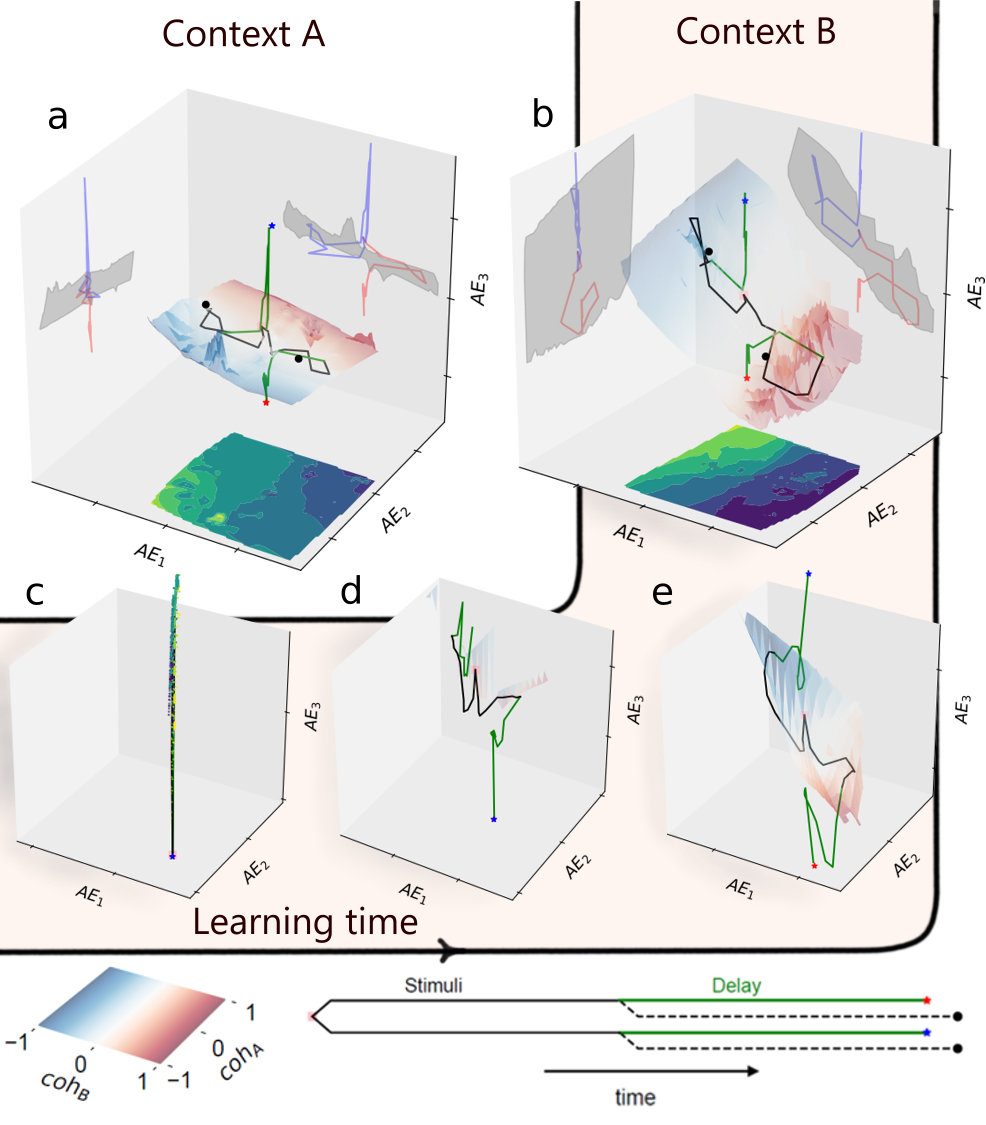
\includegraphics[width=0.85\textwidth]{images/rnn/fig_ae.png}
\caption{Формирование гибридной аттракторной архитектуры в ходе обучения с подкреплением.
(a,\,b)~Траектории в латентном пространстве для проб с противоположной когерентностью (чёрные~--- стимульный период, зелёные~--- период задержки, звёзды~--- аттракторы решений).
(c--e)~Эволюция пространства состояний: необученная сеть~(c), промежуточный этап~(d), полностью обученная сеть~(e). Решения кодируются дискретными неподвижными точками, стимул~--- непрерывным многообразием.
По~\cite{Kononov2025}.}
\label{fig:rnn_ae}
\end{figure}

\textit{Самоорганизация функциональных популяций.} Обучение с подкреплением приводило к формированию четырёх функциональных популяций: $\mathrm{G}_s$ (молчащие), $\mathrm{G}_+$ и $\mathrm{G}_-$ (селективные к положительной и отрицательной когерентности) и $\mathrm{G}_a$ (активные при любом стимуле). Характерной чертой ОП-сетей являлся баланс размеров противоположных популяций: $|\mathrm{G}_+| \approx |\mathrm{G}_-|$. В сетях, обученных ОУ, наблюдался значительный дисбаланс (отношение $|\mathrm{G}_+|/|\mathrm{G}_-|$ варьировалось от 0,5 до 2,0). Было показано, что скачок точности с плато 0,5 совпадает с бифуркацией динамики решений в бистабильную систему и появлением селективных популяций $\mathrm{G}_+$ и $\mathrm{G}_-$.

\textit{Информационно-теоретическая валидация.} Анализ взаимной информации на уровне отдельных нейронов подтвердил функциональные роли динамически определённых популяций и выявил тонкую внутреннюю структуру популяции $\mathrm{G}_a$ (секция~\ref{sec:intense_rnn}).

\textit{Структура весов.} Анализ матрицы рекуррентных весов, упорядоченной по популяциям (рис.~\ref{fig:rnn_task}\,g), выявил архитектуру типа <<победитель получает всё>> (winner-take-all): сильные положительные связи (возбуждение) внутри каждой селективной популяции ($\mathrm{G}_+ \to \mathrm{G}_+$, $\mathrm{G}_- \to \mathrm{G}_-$) и отрицательные связи (торможение) между ними ($\mathrm{G}_+ \to \mathrm{G}_-$ и наоборот). Эта структура связности не была задана заранее, а возникла спонтанно в процессе обучения.

Таким образом, поведенческая эквивалентность не означает механистической эквивалентности: при одинаковой точности обучение с подкреплением и обучение с учителем приводят к качественно различным внутренним вычислительным стратегиям. ОП формирует богатую динамическую архитектуру с квазипериодическими аттракторами и сбалансированными популяциями, тогда как ОУ предпочитает более простые решения на основе неподвижных точек.

\FloatBarrier
